\documentclass[10pt, a4paper]{beamer}

\usetheme{Berkeley}
\usecolortheme{sidebartab}
\usepackage{array}
\begin{document}
    \setbeamertemplate{sidebar left}{}
    \title{Progress Presentation-I}
    \subtitle{e-Yantra Summer Intership-2016 \\ Statechart Based Modeling of a System and Code Generation}
    \author{Mukesh Prajapati\\Rohit D Khuspe\\
    Mentor:\\ Naveen Cherupally}
    \institute{IIT Bombay}
    \date{\today}
    %\addtobeamertemplate{sidebar left}{}{\includegraphics[scale = 0.3]{logowithtext.png}}
    \frame{\titlepage}

\setbeamertemplate{sidebar left}[sidebar theme]
\section{Overview of Project}
\begin{frame}{Overview of Project}
    \begin{itemize}
        \item Project Name : Statechart Based Modeling of System and Code Generation 
        \item Objective : To create models of different tasks and generate a code using YAKINDU or QM modeling tool or KSE tool.
        \item Deliverables :
        \begin{itemize}
            \item  Folder containing all the  statechart models designed for various tasks.
            \item Report
        \end{itemize}
       
    \end{itemize}
\end{frame}

\section{Overview of Task}
\begin{frame}{Overview of Task}
    
\begin{center}
\begin{tabular}{ | m{.5cm} | m{5cm}| m{2cm} | } 
\hline
Sr No. & TASKS & DEADLINES \\ 
\hline
1. & Syntax and Symantics of statecharts & week 1  \\ 
\hline
2.& Understand the existing standard models of some systems & 3 Days\\ 
\hline
3. & Model some of the tasks & 10 Days  \\ 
\hline
4. & Explore statechart editor tool YAKINDU and KSE.  & 3 Days  \\ 
\hline
5. & Implement the model in KSE tool using liveness formulas or GUI  & 7 Days  \\ 
\hline
6. & Generate the code from the implemented model & 4 days  \\ 
\hline
7. & Make Report & 5 Days\\
\hline
\end{tabular}
\end{center}
\end{frame}

\section{Task Accomplised}
\begin{frame}{Task Accomplised}
    \begin{itemize}
        \item Learnt Syntax and Semantics of Statecharts.
            \begin{itemize}
            \item What are Statecharts?
            \item Its features.
            \begin{itemize}
                \item Clustering \\
                In statecharts we represent every possible state of a system. It might happen that a particular state contains more than one substates and transition takes place from this substates to a respective state on an occurance of particular event.\\
                \begin{figure}[h]
                \centering
                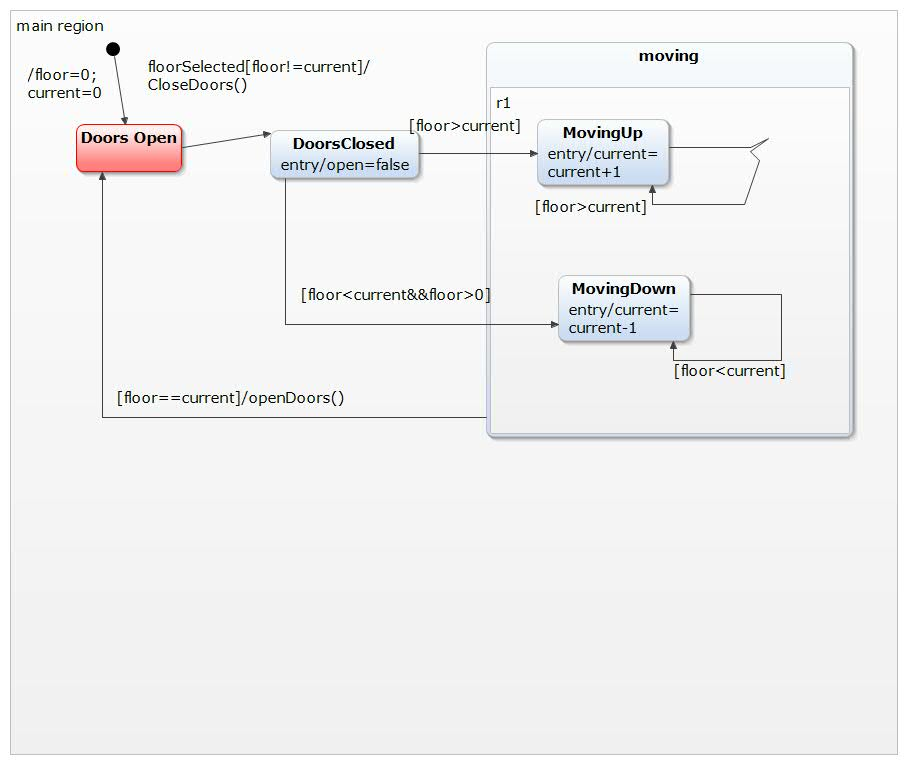
\includegraphics[width=9cm,height=8cm]{elevator.jpg}
                \end{figure}
                \end{itemize}
                \end{itemize}
                \end{itemize}
                \end{frame}
                 \section{Task Accomplised}
              \begin{frame}
                \begin{itemize} 
                 \item Orthogonality\\
           Orthogonality means AND decomposition of states.\\
           \begin{figure}[h]
                \centering
                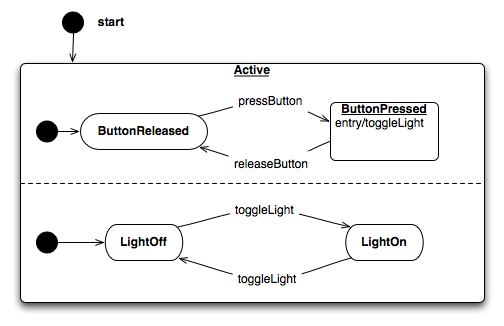
\includegraphics[width=3cm,height=3cm]{switch.png}
                \end{figure}
            \item Condition and Selection Entrance.
            Upon the entrance of the superstate a condition is checked and the transition is made to one of the sub-states in the superstate.\\
            The transition is made depending on the generic value of the input rather than the condition.\\
            \end{itemize}
            \end{frame}
            \begin{frame}
            \begin{figure}[h]
                \centering
                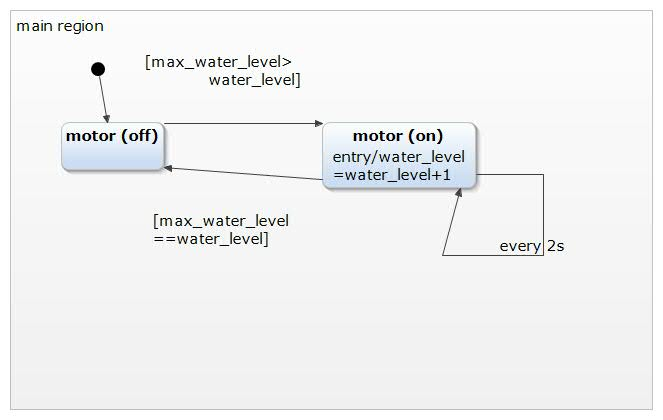
\includegraphics[width=5cm,height=3cm]{water.jpg}
                \end{figure}
                \begin{figure}[h]
                \centering
                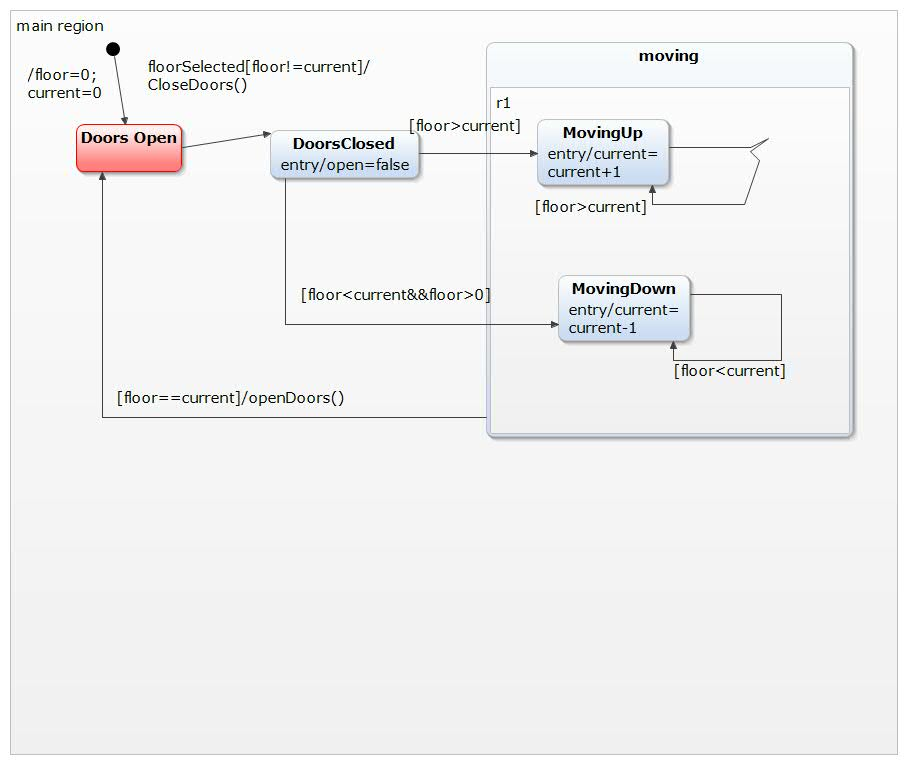
\includegraphics[width=7cm,height=5cm]{elevator.jpg}
                \end{figure}
                \end{frame}
                \begin{frame}
                \begin{itemize}
                \item Significance of History\\
                History means entering the state most resently visited.\\
                \begin{figure}[h]
                \centering
                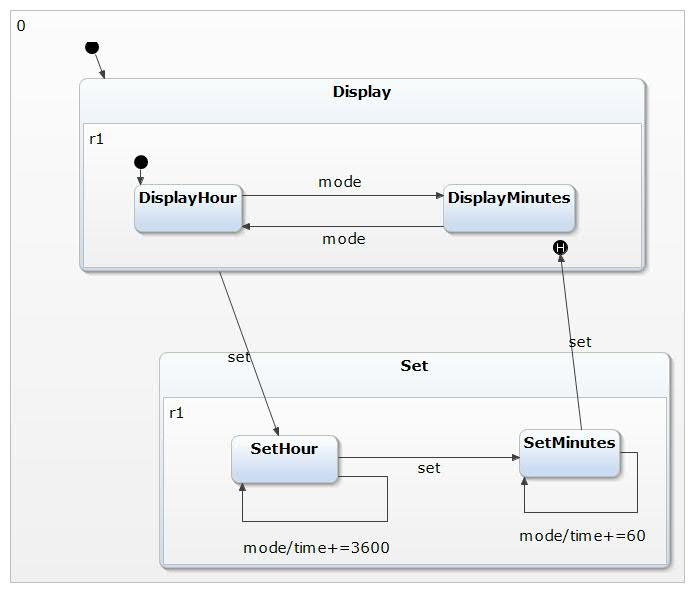
\includegraphics[width=7cm,height=5cm]{clock.jpg}
                \end{figure}
                \end{itemize}
                \end{frame}
                \begin{frame}
            \begin{itemize}
           \item Understood the valet parking robot model using statecharts.
            \item Explored the statechart editor tools YAKINDU and QM modeling tool.
        \item Modeled some tasks.
    \end{itemize}
\end{frame}


\section{Challenges Faced}
\begin{frame}{Challenges Faced}
    \begin{itemize}
        \item \textbf{Issue} : To find appropriate software for modeling a task.
        \item To find appropriate software for code generation.
        \item  Understand the generated code and how to make the code Firebird V platform dependent.
        \end{itemize}
\end{frame}

\section{Future Plans}
\begin{frame}{Future Plans}
    \begin{itemize}
    \item Model the e-YANTRA competition project using statechart.
        \item  Learn the KSE tool.
         \item    Generate the platform independent code using either KSE or Yakindu or QM.
         \item    Make the platform independent code compatible with firebird V.
          \item   Report.

    \end{itemize}
\end{frame}


\section{Thank You}
\begin{frame}{Thank You}
    \centering THANK YOU !!!
\end{frame}
\end{document}